\documentclass[12pt,fleqn,a4paper]{article}

\usepackage{latexsym}
\usepackage{url}
\usepackage{xspace}
\usepackage{epsfig}
\usepackage{psfrag}
\usepackage{a4wide}
\usepackage{marvosym}
\usepackage{amsmath,amsfonts,amssymb,amsthm,latexsym}
\usepackage{graphics,graphicx,color,subfigure}
\usepackage{fancyhdr}
\usepackage{algorithm}
\usepackage{algorithmic}
\usepackage[english]{babel}
\usepackage[latin1]{inputenc}

\textheight 680pt
\textwidth 460pt
\topmargin -40pt
\oddsidemargin 5pt
\evensidemargin 5pt
\parindent 0pt

\pagestyle{fancyplain} \setlength{\headheight}{16pt}
\renewcommand{\sectionmark}[1]{\markright{\thesection\ #1}}
\lhead[\fancyplain{}{\thepage}]
    {\fancyplain{}{\rightmark}}
\rhead[\fancyplain{}{\leftmark}]
    {\fancyplain{}{\thepage}}
\cfoot{}
\renewcommand{\thesection}{\arabic{section}}
\renewcommand{\thesubsection}{\arabic{section}.\arabic{subsection}}


\begin{document}
\begin{titlepage}%Institution
\vspace{2cm}
\centerline{
\large{Department of Artificial Intelligence and Human Interfaces}}
\vspace{0.2cm}
\centerline{\large{University of Salzburg}}%Optimizing Activation Function Distribution using Evolutionary Algorithms
%\hline
\vspace{2cm}

\centerline{\large{PS Natural Computation}}
\centerline{SS 24}
\vspace{1cm}

\centerline{\Large{\bf{Title}} }%Type of the Document
\vspace{1cm}

\vspace{0.4cm}%Date
\centerline{\today}
\vspace{5cm}%Authors

%\hline
\vspace{0.2cm}
Project Members:\\
\centerline{Ante Krajnovic, 12244629, ante.krajinovic@stud.plus.ac.at}\\
\centerline{Khalil Ibrahim, 11803004, khalil.ibrahim2@stud.plus.ac.at}\\
\centerline{Mitsuhiro Kitajima, 12314106, mitsuhiro.kitajima@stud.plus.ac.at}\\
\centerline{Peter Balint, 12213073, peter.balint@stud.plus.ac.at}\\
\centerline{\ldots}
\vspace {1cm}\\

Academic Supervisor: \\
\centerline{Helmut MAYER}
\centerline{helmut@cosy.sbg.ac.at}
\vspace{1.5cm}\\
Correspondence to: \\
\centerline{Universit\"{a}t Salzburg} \\
\centerline{Fachbereich AIHI} \\
\centerline{Jakob--Haringer--Stra\ss e 2} \\
\centerline{A--5020 Salzburg} \\
\centerline{Austria}
\clearpage
\end{titlepage}

%Table of Content
% \setcounter{page}{1}
% \pagenumbering{Roman} %I,II,III... in the TOC
% \tableofcontents

\clearpage
\pagestyle{headings}
\pagenumbering{arabic}  %Better if TOC is variable (more than one page)
\setcounter{page}{1}
\pagenumbering{arabic}  %Better if TOC is variable (more than one page)
\setcounter{page}{1}

\abstract{This is a report for the Natural Computation class of Prof. Mayer
in 2026, discussing optimization of activation function distribution using
evolutionary algorithms in an artificial neural network.}

\section{Introduction}

In a typical artificial neural network, usually only one activation function
is used for all neurons.  However, it is also possible to encode a different
activation function for every neuron, with the hope that better results can
be achieved.  The distribution of the activation functions in this case is a
good target for optimization.

Our group has been assigned the task of performing this optimization in a
basic artificial neural network by means of a basic evolutionary algorithm.
Our experiments will be performed on benchmarks and data provided by the
"basics" group.  We use the PyTorch framework for our work.

In a genetic algorithm, there is a set of individuals that are then mutated
and discarded in each iteration.  In this case, an individual is defined as
the assignment of activation functions in the neural network's hidden layer.

First, the initial generation is chosen as a random list of activation
function vectors from a fixed set of activation functions.  Then, for each
generation, training on a single set of weights $W$ is performed using each
individual of the population.  The weights are kept in the next generation,
with only the population being changed.

Population of the next generation is decided using a semi-random selection
of two highly fitting individuals and then optionally combining these.
Finally, the resulting function is randomly mutated.  The experiment may
be considered successful if, after a number of such generations, the
resulting activation function distribution performs better than a network
with a uniform activation function.

\newpage

\section{Milestones} % NOT in final paper
\begin{itemize}
\item{Familiarize ourselves with topic. Until: 25.03.2026}
\item{Experiment with assigning individual activation functions per neuron
and modifying this assignment, based on experimential data of the basics
group.  Until: 06.05.2026}
\item{Experiment with using an evolutionary algorithm to adjust the
activation functions. Until: 20.05.2026}
\item{Create a framework for evaluation of evolutionary algorithms in this
context.  Until: 03.06.2026}
\item{Experiment with different evolutionary algorithms. Until: 17.06.2026}
\item{Finalize report. Until: TBA}
\end{itemize}

\newpage

\section{Progress of Work} % NOT in final paper

\subsection{Week 1, Wednesday, 04.03.2026}

Lecture introduction.

\subsection{Week 2, Wednesday, 11.03.2026}

Proseminar introduction.

\subsection{Week 3, Wednesday, 25.03.2026}

First presentation: introduction to the topic.  (By Khalil)

\subsection{Week 4, Wednesday, 22.04.2026}

Second presentation: assignment of responsibilities, organization.

\subsection{Week 5, Wednesday, 06.05.2026}
Third presentation: Activation Functions (By Khalil)

\subsection{Week 6, Wednesday, 20.05.2026}

\subsection{Week 7, Wednesday, 03.06.2026}

\subsection{Week 8, Wednesday, 17.06.2026}

\subsection{Week 9, Wednesday, 24.06.2026}

(?)

\newpage

\section{Subproject Responsibilities} % NOT in final paper

\begin{itemize}
\item Research prior art/references: Khalil Ibrahim
\item Research possible (modern) activation functions: Khalil Ibrahim
\item Implement assignment of AFs to individual neurons in PyTorch: Peter Balint
\item Research/design a possible evolutionary algorithm (for AF optimization): Mitsuhiro Kitajima
\item Implement the evolutionary algorithm in PyTorch: Peter Balint
\item Experiment with different evolutionary algorithms (selection, mutation, etc.): Ante Krajinovic
\item Charts: Ante Krajinovic
\item Report, editing: Peter Balint
\end{itemize}

\newpage
\section{Activation Functions}

Activation functions determine how strongly a neuron ``fires'' and are a fundamental component of artificial neural networks. Their primary role is to introduce non-linearity into the model. Without activation functions, a neural network, regardless of its depth, would collapse into a purely linear function.

Therefore, activation functions are essential for both learning capability and overall performance of neural networks.

\subsection{Classical Activation Functions}

One of the earliest and most commonly used activation functions is the \textbf{sigmoid} function. It maps input values into the range $(0, 1)$. However, sigmoid suffers from saturation for large positive or negative inputs, which leads to vanishing gradients and consequently slow learning.

\begin{equation}
\sigma(x) = \frac{1}{1 + e^{-x}}
\end{equation}

Another classical function is \textbf{tanh}, which outputs values in the range $(-1, 1)$. Compared to sigmoid, tanh is generally more effective due to its zero-centered output, but it also suffers from saturation problems.
\begin{equation}
\tanh(x) = \frac{e^{x} - e^{-x}}{e^{x} + e^{-x}}
\end{equation}

The step function is a historical activation function that outputs either 0 or 1. It is no longer used in modern neural networks because it is not differentiable and therefore incompatible with gradient-based optimization methods.
\begin{equation}
f(x) =
\begin{cases}
1 & \text{if } x \geq 0 \\
0 & \text{if } x < 0
\end{cases}
\end{equation}

A major breakthrough was the introduction of the \textbf{ReLU} (Rectified Linear
Unit) function:

\begin{equation}
f(x) = \max(0, x)
\end{equation}

ReLU is computationally efficient and significantly improves training speed and stability. However, it introduces the so-called \textit{dying ReLU} problem, where neurons can become permanently inactive.

\subsection{Modern Activation Functions}

To address limitations of classical approaches, several modern activation functions have been proposed.

\textbf{Leaky ReLU} introduces a small negative slope for negative inputs, preventing dead neurons.

\begin{equation}
f(x) =
\begin{cases}
x & \text{if } x \geq 0 \\
\alpha x & \text{if } x < 0
\end{cases}
\end{equation}

\textbf{PReLU} extends Leaky ReLU by making the negative slope a learnable
parameter.

\begin{equation}
f(x) =
\begin{cases}
x & \text{if } x \geq 0 \\
a x & \text{if } x < 0
\end{cases}
\quad \text{where } a \text{ is learnable}
\end{equation}

\textbf{ELU} (Exponential Linear Unit) provides a smoother transition for negative values and improves training stability.

\begin{equation}
f(x) =
\begin{cases}
x & \text{if } x \geq 0 \\
\alpha (e^{x} - 1) & \text{if } x < 0
\end{cases}
\end{equation}

\textbf{Swish}, introduced by Google, is defined as:

\begin{equation}
f(x) = x \cdot \sigma(x)
\end{equation}

It has shown strong empirical performance in deep learning models.

\textbf{GELU} (Gaussian Error Linear Unit) is widely used in transformer
architectures such as BERT and GPT and provides smooth gradient behavior,
especially in large-scale models.  Following is an approximation of the
function:

\begin{equation}
f(x) \approx 0.5x \left(1 + \tanh\left(\sqrt{\frac{2}{\pi}}(x + 0.044715x^3)\right)\right)
\end{equation}

\textbf{Mish} is a more recent activation function characterized by high smoothness and strong information preservation properties, often improving performance in deep networks.

\begin{equation}
f(x) = x \cdot \tanh(\ln(1 + e^{x}))
\end{equation}

\begin{figure}[h]
    \centering
    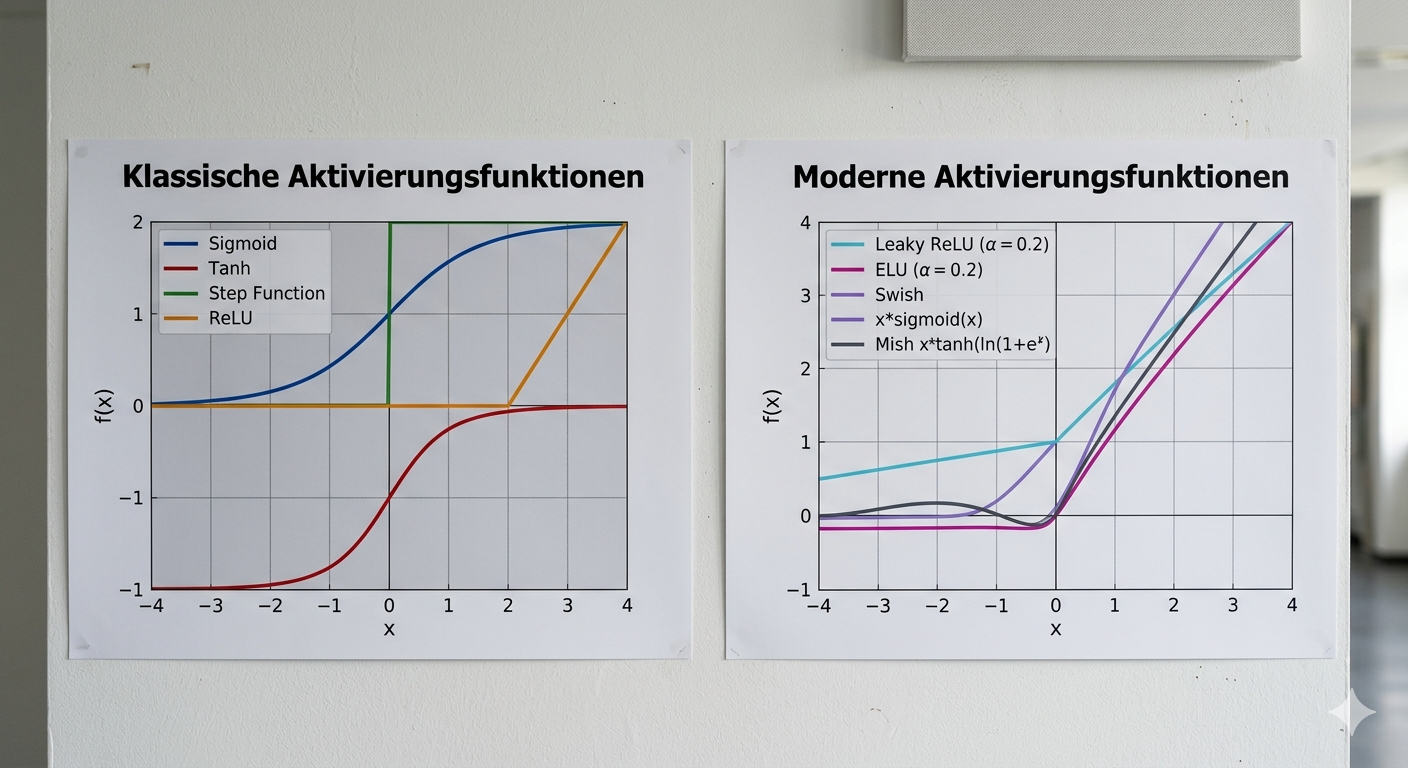
\includegraphics[width=0.5\textwidth]{classic&mod.png}
    \caption{Visual representation of traditional (left) versus modern (right) activation functions.}
    \label{fig:meinbild}
\end{figure}

\subsection{Motivation for New Activation Functions}

Classical activation functions suffer from several well-known issues:

\begin{itemize}
    \item Vanishing gradients
    \item Poor gradient flow
    \item Unstable training behavior
\end{itemize}

Modern activation functions aim to overcome these limitations by improving:

\begin{itemize}
    \item Training stability
    \item Generalization performance
    \item Convergence speed
\end{itemize}

\newpage
\section{Experimental Results}

To evaluate the effectiveness of the evolutionary optimization, each benchmark
(Easy, Medium, and Hard) was executed ten times. Only the final evolved
activation function distributions were considered for the evaluation. Baseline
runs marked as \textit{"functions not fixed"} were excluded from the analysis.

\subsection{Average Test Accuracy}

Table1 summarizes the average test accuracy achieved for
each benchmark.

\begin{table}[h]
\centering
\begin{tabular}{lcc}
\hline
Problem & Number of Runs & Average Test Accuracy \\
\hline
Easy   & 10 & 91.40\% \\
Medium & 10 & 97.45\% \\
Hard   & 10 & 52.15\% \\
\hline
\end{tabular}
\caption{Average test accuracy over ten evolutionary runs.}
\label{tab:avg_accuracy}
\end{table}

The evolutionary search consistently achieved excellent performance on the
Easy and Medium benchmark problems. In particular, the Medium dataset reached
an average test accuracy of 97.45\%, indicating that heterogeneous activation
function assignments can successfully optimize network performance. The Hard
benchmark remained considerably more challenging, reaching an average accuracy
of only 52.15\%.
\newpage
\subsection{Distribution of Activation Functions}

To better understand which activation functions were preferred by the
evolutionary algorithm, all activation assignments from the ten optimized runs
were aggregated.

\begin{table}[h]
\centering
\begin{tabular}{lrrrrrrr}
\hline
Problem & Identity & ReLU & GELU & Tanh & SiLU & Sigmoid & Total \\
\hline
Easy   & 36 & 12 & 8 & 9 & 8 & 7 & 80 \\
Medium & 40 & 26 & 46 & 25 & 8 & 15 & 160 \\
Hard   & 44 & 52 & 75 & 51 & 51 & 47 & 320 \\
\hline
\end{tabular}
\caption{Absolute frequency of evolved activation functions.}
\label{tab:function_counts}
\end{table}

Since the network architectures contain different numbers of hidden neurons,
the relative frequency of each activation function provides a more meaningful
comparison.

\begin{table}[h]
\centering
\begin{tabular}{lrrrrrr}
\hline
Problem & Identity & ReLU & GELU & Tanh & SiLU & Sigmoid \\
\hline
Easy   & 45.00\% & 15.00\% & 10.00\% & 11.25\% & 10.00\% & 8.75\% \\
Medium & 25.00\% & 16.25\% & 28.75\% & 15.63\% & 5.00\% & 9.38\% \\
Hard   & 13.75\% & 16.25\% & 23.44\% & 15.94\% & 15.94\% & 14.69\% \\
\hline
\end{tabular}
\caption{Relative distribution of evolved activation functions.}
\label{tab:function_percentages}
\end{table}

The Easy benchmark strongly favored the Identity activation function, which
accounted for 45\% of all selected activations. In contrast, the Medium and
Hard benchmarks exhibited a clear preference for GELU, representing 28.75\%
and 23.44\% of all evolved activation functions, respectively. While the Hard
benchmark still preferred GELU, the remaining activation functions were
distributed much more evenly, suggesting that more difficult problems benefit
from a heterogeneous mixture of activation functions rather than relying on a
single dominant choice.

\subsection{Summary Comparison}

Classical activation functions are simple and computationally efficient but limited in deep architectures. In contrast, modern activation functions are smoother, more stable, and often adaptive or learnable, making them more suitable for deep learning applications.

% EA design and description part
\newpage
\section{Design of Evolutional Algorithm}
\subsection{Overview}
In this section, we describe how we have designed the evolutionary algorithm for
optimizing the distribution of activation functions in the hidden layer(s) of a neural network.
As an assumption, we consider a neural network with one or more hidden layers.
Let \(v=\{v_1, v_2, \dots, v_n\} \) be a raw output of the hidden layer and 
\(f = \{f_1, f_2, \dots, f_n\}\) be the activation functions applied to each neuron in the hidden layer, respectively,
where \(f_i \in \mathcal{F}\) for \(i=1,\dots,n\) and \(\mathcal{F}\) is the set of activation functions (we call \(\mathcal{F}\) the ``function pool'').
\subsection{Algorithm}
We use a simple genetic algorithm for the optimization.
For the sake of simplicity, the algorithm assumes a single hidden layer for a neural network. For a neural network with $N>1$ layers, we use either concatenated activation function layers as an individual, or another method that fits better.

\begin{algorithm}[H]
\caption{Optimization of Activation Function Distribution}
\label{alg:optimization}
\begin{algorithmic}[1]
\REQUIRE Population $P$ of size $M$, function pool $\mathcal{F} = \{f_1, \dots, f_n\}$, max generations $g$
\STATE Initialize $P^0$ with random functions from $\mathcal{F}$ for each individual $i \in \{1,\dots,M\}$
\STATE Initialize $f_{best}$
\STATE 
\FOR{$t = 0$ to $g$}
    \FOR{$i = 1$ to $M$}
        \STATE Evaluate fitness of $P^t_i$ by training NN with $P^t_i$
        \IF{$fitness(P^t_i) > fitness(f_{best})$}
            \STATE $f_{best} = P^t_i$
        \ENDIF
    \ENDFOR
    \STATE Select new population $P^{t+1}$ from $P^t$ using selection operator
    \STATE Mutate $P^{t+1}$ using mutation operator
\ENDFOR
\RETURN $f_{best}$
\end{algorithmic}
\end{algorithm}
\subsection{Proposal of Operators}
\subsubsection{Selection}
For the selection of individuals from the current generation $P^t$ to the next generation $P^{t+1}$, we use a combination of elitism and tournament selection. We initially set $k=2$, meaning the selection process involves 4 randomly selected individuals from $P^t$.
\begin{algorithm}[H]
\caption{Selection($k$)}
\label{alg:selection}
\begin{algorithmic}[1]
\STATE Select $f_{best}\in P^t$
\STATE Add $f_{best}$ to $P^{t+1}$ 
\WHILE{$P^{t+1}$ is not full}
\STATE Select $k$ individuals from $P^t$ uniformly at random 
\STATE Set the best fitting individual as $f_A$
\STATE Select $k$ individuals from $P^t$ uniformly at random again
\STATE Set the best fitting individual as $f_B$
\STATE Execute $Crossover(f_A, f_B)$ with probability $p_c$
\IF {Crossover is executed}
\STATE Add $f_C$ to $P^{t+1}$
\ELSE \STATE Add $\max_{fitness(f)}\{f_A, f_B\}$ to $P^{t+1}$
\ENDIF
\ENDWHILE
\end{algorithmic}
\end{algorithm}
\subsubsection{Crossover}
We use uniform crossover. The algorithm takes two parents as input and returns one child. 
The probability of crossover is initially set to $0.8$. Although this probability may be varied in experiments, it will remain high.
\begin{algorithm}[H]
\caption{Crossover($f_A, f_B$)}
\label{alg:crossover}
\begin{algorithmic}[1]
\STATE Initialize $f_C$
\FOR{each $({f_A}_i,{f_B}_i)$ in $f_A, f_B$}
\STATE ${f_C}_i = {f_A}_i$ with probability $0.5$
\STATE Otherwise, ${f_C}_i = {f_B}_i$
\ENDFOR
\RETURN $f_C$
\end{algorithmic}
\end{algorithm}
\subsubsection{Mutation}
Mutation is implemented in the form of randomly drawing functions from the function pool to replace selected elements in an individual.
The probability of mutation is initially set to $0.01$. Although this probability may be varied in experiments, it will remain very low. The number of mutated elements, $l$, is set to approximately 20\% of the length of the individual.
\begin{algorithm}[H]
\caption{Mutation($f, l$)}
\label{alg:mutation}
\begin{algorithmic}[1]
\STATE Select $l$ elements from $f$ uniformly at random
\FOR {each selected element $f_i$}
\STATE Replace $f_i$ with a randomly selected $f_s \in \mathcal{F}\setminus\{f_i\}$
\ENDFOR
\end{algorithmic}
\end{algorithm}


\newpage

% links go here, NOT in references
\section{Links}

\begin{itemize}
\item Project Page: \url{http://student.cosy.sbg.ac.at/~pbalint/nc/}
\item PS Page:
\url{http://www.cosy.sbg.ac.at/~helmut/Teaching/PSRobotik/}

\end{itemize}


% real scientific references
\bibliography{}		% .bib files here

\section{References}

\begin{itemize}
    \item Goodfellow et al. (2016): \textit{Deep Learning}
    \item Nair \& Hinton (2010): ReLU
    \item Maas et al. (2013): Leaky ReLU
    \item Clevert et al. (2015): ELU
    \item Ramachandran et al. (2017): Swish
    \item Hendrycks \& Gimpel (2016): GELU
    \item  Mish Activation Function (2019): Misra 
\end{itemize}

\end{document}
